\documentclass[10pt,a4paper]{article}

\usepackage[a4paper,hmargin=2.5cm,vmargin=3cm] {geometry}
\usepackage{fix-cm}
\usepackage{amsmath,amssymb,amsthm}
\usepackage{tikz}
\usepackage{graphicx}
\usepackage[polish,english]{babel}
\usepackage[T1]{fontenc}
\usepackage[utf8]{inputenc}
\usepackage{url}
\usepackage{verbatim}
\usepackage{color}
\usepackage{ae}
\usepackage[ruled]{algorithm}
\usepackage{algorithmicx}
\usepackage{algpseudocode}
\usepackage[breaklinks]{hyperref}
\usepackage[polish,english]{babel}
\usepackage{multirow}
\usepackage{epstopdf}
\usepackage{listings}
\usepackage{caption}
\usepackage{subcaption}

\newtheorem{theorem}{Theorem}
\newtheorem{lemma}{Lemma}

\definecolor{myRed}{rgb}{0.9,0.3,0.1}
\newcommand{\pawel}[1]{\noindent\colorbox{myRed}{Pawel: #1}}
\definecolor{myYellow}{rgb}{0.99,0.99,0.05}
\newcommand{\jarek}[1]{\noindent\colorbox{myYellow}{Jarek: #1}}
\newcommand{\todo}[1]{\noindent\colorbox{myRed}{TODO: #1}}
\DeclareMathOperator{\rightSon}{right}
\DeclareMathOperator{\leftSon}{left}

\newcommand{\Oh}{\mathcal{O}}
\newcommand\bigforall{\mbox{\Large $\mathsurround0pt\forall$}} 

\begin{document}

%%%%%%%%%%%%%%%%%%%%%%%%%%%%%%%%%%%%%%%%%%%%%%%%%%

\pagenumbering{roman}

\topmargin-20pt
\oddsidemargin0pt
\evensidemargin0pt
\textheight660pt
\textwidth445pt

\selectlanguage{polish}
\begin{titlepage}
\Large

\begin{center}

\textbf{\large%
Uniwersytet Wrocławski\\
Wydział Matematyki i Informatyki\\
Instytut Informatyki}


\vspace{4cm}
Jarosław Gomułka 

\vspace{0.5cm}
\textbf{%\normalsize%
Shuffla: fast and scalable full-text search engine}

\end{center}

\vspace{7cm}
\begin{flushright}
\begin{minipage}[c]{6.2cm}
  Praca magisterska\\
  napisana pod kierunkiem\\
  dr. Pawła Gawrychowskiego
\end{minipage}
\end{flushright}

\vfill

\begin{center}
 Wrocław 2012
\end{center}

\newpage

\end{titlepage}

\newpage

\thispagestyle{empty}

\Large

~\vfill
Oświadczam, że pracę magisterską wykonałem samodzielnie i zgłaszam ją do oceny.

\vspace{2cm}
Data: \dotfill\quad Podpis autora pracy: \dotfill


\vspace{4cm}
Oświadczam, że praca jest gotowa do oceny przez recenzenta.

\vspace{2cm}
Data: \dotfill\quad Podpis opiekuna pracy: \dotfill

\normalsize

\restoregeometry
%%%%%%%%%%%%%%%%%%%%%%%%%%%%%%%%%%%%%%%%%%%%%%%%%%

\newpage
\thispagestyle{empty}

\begin{abstract}
Celem tej pracy jest stworzenie efektywnego i skalowalnego narzędzia do dokładnego przeszukiwania zbioru użytkowników dużego portalu społecznościowego. 

Jednym z możliwych rozwiązań tak postawionego problemu jest zastosowanie jednej z popularnych relacyjnych baz danych. Inną możliwością jest użycie wyszukiwarki tekstowej takiej jak Apache Solr czy Sphinx Search. Jeszcze innym pomysłem jest zaimplementowanie własnego narzędzia. Celem tej pracy jest przedstawienie Shuffli, wyspecjalizowanej wyszukiwarki stworzonej przeze mnie z myślą o tym konkretnym problemie. Oprócz przedstawienia architektury i szczegółów implementacji, porównam jej efektywność z PostgreSQL, Apache Solr, oraz Sphinx Search.

\bigskip
Pracuję nad portalem nk.pl (który jest największym polskim portalem społecznościowym) od początku roku 2011. W sierpniu 2011 roku zostało mi powierzone rozwiązanie tego problemu.

\bigskip
\noindent \textbf{Słowa kluczowe:} bazy danych, nosql
\end{abstract}

\selectlanguage{english}
%%%%%%%%%%%%%%%%%%%%%%%%%%%%%%%%%%%%%%%%%%%%%%%%%%


\title{Shuffla: fast and scalable full-text search engine}
\author{Jarosław Gomułka}

\maketitle

\pagenumbering{arabic}
%%%%%%%%%%%%%%%%%%%%%%%%%%%%%%%%%%%%%%%%%%%%%%%%%%

\section{Introduction}

Given a list of people (their first name, last name, age, home town) we want to provide highly available, scalable and very fast solution that can search through such data.

One possible solution is to use relational database. Other solution is to use a full-text search engine like Apache Solr or Sphinx Search. Another solution is to develop our own specialized search engine dedicated to solving such tasks. In this paper I will describe Shuffla, a full-text search engine created by me and compare it to Sphinx, Solr, and PostgreSQL. 

I have been working at nk.pl (the biggest Polish social networking website) since the beginning of 2011. In August 2011 I was appointed to solve the task described above. 

\begin{figure}[h!]
\centering
  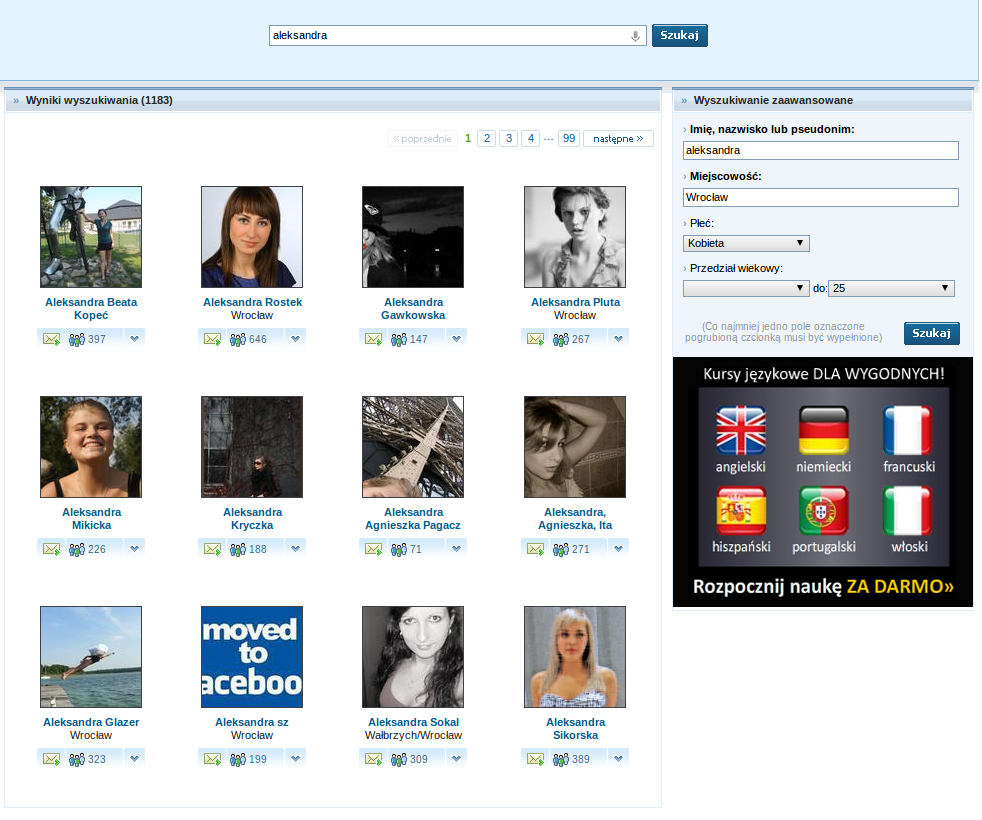
\includegraphics[width=12cm]{nk_search}
  \caption{Searching users in nk}
  \label{fig:nk_search}
\end{figure}

\section{Problem definition}

\subsection{Database model}

As with many databases, Shuffla allows you to store different types of objects. Like SQL, Shuffla does it by offering possibility of creating multiple tables. A table might be defined as a combination of a table name and a list of pairs <column name, type of column>. Fields in out model table are first name, last name, age, home town. They are strings and numbers; therefore a type of column can be either a string or a number.

\subsection{Selecting data}

Shuffla like every other database offers possibility of searching data. There are different possible conditions for different types. Possible conditions for numbers are equality check, inequalities and strict inequalities. Strings are compared using lexicographic order so equality check, inequalities and strict inequalities should be supported. There are two additional conditions
\begin{enumerate}
\item Checking if a given string is a prefix of the selected column value.
\item Checking if a given string is a substring of the selected column value. 
\end{enumerate}

Users can define \verb|order_by| column. If the \verb|order_by| clause is specified, the returned rows are sorted in the specified order. Size of the results may be narrowed by defining \verb|offset| and \verb|limit|. These search parameters must work exactly in the same way as their equivalents in SQL.

Furthermore, it should be possible to personalize the order of the results. For example, if a user from San Francisco is looking for Jane, the top results should show Janes from San Francisco, then Janes from California, then the rest of U.S. GPS coordinates may be fetched by the modern web browsers \cite{FETCHGPS}. GPS coordinates can be added to the scheme. To selecting users in some range we can add conditions   
\begin{enumerate}
\item{someLatitiude - radius $\leq$ latitude $\wedge$ latitude $\geq$ someLatitude + radius}
\item{someLongitude - radius $\leq$ longitude $\wedge$ longitude $\geq$ someLongitude + radius}
\end{enumerate}

\section{Shuffla's competition}
The problem described in this paper may be solved by various existing software. There are two most common kinds of software which can be used: relational databases and full-text search engines.

\subsection{Relational databases}
Relational Database Management System data is structured in database tables, records and fields. Each table contains multiple rows. Each row contains multiple fields. Relational Databases store data in collection of tables, which might be related by common fields. They also provide relational operators to manipulate the data stored in those tables. Most relational databases use SQL as query language. The most popular relational databases are PostgreSQL, MySQL, MSSQL Server. In this paper I will only test PostgreSQL which is in my opinion best relational database nowadays.

\subsubsection{PostgreSQL}
PostgreSQL has really useful features such as: point-in-time recovery, asynchronous replication, online/hot backups, a sophisticated query planner/optimizer and write ahead logging for fault tolerance. It supports international character sets, unicode, and is locale-aware for sorting and case-sensitivity. It is highly scalable both in the quantity of data it can manage and in the number of concurrent users it can accommodate. PostgreSQL keeps its data on a disk and it implements their own master-slave replication. There are also few middlewares which could provide master-master replication \cite{PSQLREPL}. PostgreSQL performance can be easily monitored by software like Munin and New Relic. SQL implies very strong typing system. PostgreSQL processes comparisons and inequalities very fast as long as proper indexes are created. Serious disadvantage of using PostgreSQL for this problem is performance on substring queries; B-tree based indexes do not support fast processing of substring queries. There are attempts to create full-text indexes (gist, gin) which could outperform classical index based on B-tree.
Here is a brief example of processing query by B-tree: \verb|first name = John| \verb|and| \verb|substring(last name) = qwertyabc| \verb|and| \verb|limit = 1|. In this case engine finds first person with first name John. It takes $\Oh(\log n)$ time where $n$ is number of rows in the table. Finding another person with first name John takes $\Oh(1)$. Unfortunately, all these rows must be processed one by one to check if they contain substring \verb|qwertyabc|. Since there is no one with such a name, engine will process all men named John and will find nothing.

\subsection{Full-text search engine}
In text retrieval full-text search refers to techniques for searching document or a collection in a full text database. The searches are based on parts of the original texts represented in databases. The most popular full-text search engines are Sphinx Search and Apache Solr. Almost all big players are choosing Sphinx and Solr over other engines like Elastic Search and Xapian so I am going to consider only the first two. Both engines are based on similar data structure called inverted index. Inverted index keeps list of every word occurring in database. For each word inverted index remembers where this word occurs. This is similar to glossaries which we can often see at the end of books. Such inverted index is stored on a disk. When processing query, engine selects best strategy to follow. Strategy can be seen as a procedure:
\begin{enumerate}
\item Narrow as many words as possible from inverted index which needs to be processed. 
\item Process remaining words. 
\end{enumerate}
For example, if a query is \verb|first name = John| \verb|and| \verb|limit 1|, we are only interested in word \verb|John| from inverted index. The engine finds the first occurrence and returns it. Ineqalities, prefix queries and substring queries are treated similarly to equality checks. They narrow the number of words in the dictionary that algorithm needs to process. If a query is \verb|first name = John| \verb|and| \verb|substring(last name) = qwertyabc| \verb|and| \verb|limit = 1|, it is likely that there are more Johns than all people with last name containing \verb|qwertyabc|. By using sophisticated data structure, engine may find out that the are not many people with a name containing \verb|qwertyabc|. Such output is rendered very fast\footnote{with table containing 8 million rows Solr renders output for such query in less than 0.01 second} In worst case scenario algorithm works in linear time. An example for such case could be \verb|substring(last name)=a| \verb|and| \verb|substring(last name) = b| \verb|and| ... \verb|and| \verb|substring(last name) = z| \verb|and| \verb|limit = 1|. Almost whole inverted index must be processed and the result set will be empty.

\subsubsection{Solr}

Solr is an open source search platform from the Apache Lucene project. It has lots of very handy features like faceted searches, geospatial searches, string tokenizers (makes John and Johnny to be interpreted as the same name). Solr has a great admin interface which provides extensive statistics on queries, updates and cache usage. It is easily extendable for new features. Solr implements master-slave replication which solves scalability problems. Everything is perfect except one thing. 

Solr does not modify database in real-time. Data is not added to database immediately after insert/update commands. The data is actually inserted after calling commit command. Commit is very costly operation because it requires all caches to be invalidated. Even for the table with a few entries, commit takes more than 0.1 sec. Time for commit grows with a growing size of data. An instance of Solr at nk contains +20 million entries and commit takes about 20 seconds. Commit does not block database, which is very important. After commit, search engine is in a warming stage. It means that all caches are flushed. First queries after commit can run slowly. After a number of processed queries, engine is past warming stage and queries are handled much faster.

\subsubsection{Sphinx Search}

Sphinx Search is a very good and fast search engine. Sphinx provides excellent relevance ranking (by using multiple factors like phrase proximity and various statistics). It is possible to install Sphinx as MySQL or PostgreSQL plugin. Unfortunately our specification emphasizes Sphinx disadvantages.
Sphinx does not have replication. It is unacceptable for any high traffic website. There is a way to simulate replication. Inverted index is stored on a disk. Directory containing index could be replicated by a file system (for example network file system). But if an index is big than syncing such directories would take too much time and would be inefficient and problematic.

There are several high-traffic websites with Sphinx search. They horizontally partition searched data across search nodes and then process it in parallel \cite{SPHINXPARAL}.

Replication is very important to us because in case of server failure we want to avoid downtime. This eliminated Sphinx Search from our list of potential search engines. 

Apart from replication sphinx has another problem. There are two different kinds of indexes in sphinx.
\begin{enumerate}
\item Real-time index - enables inserts
\item Normal index - modifications possible only by rebuilding the whole index (which takes too much time for our requirements)
\end{enumerate}

Real-time index has many caveats \cite{SPHINXCAV}. Prefix and substring queries are not supported yet. Periodical rebuiling of an index with more than 20 million elements is problematic. Apache Solr and Sphinx search use similar data structures. Since number of features implemented by Solr is much greater than in Sphinx I decided to look only into Solr. 

\subsection{Why am I creating new search engine?!}
It seems that none of the existing solutions process search queries very fast. In worst case scenario it is always $\Oh(n)$. All solutions work on data stored on a disk. Nowadays when RAM is cheap and servers with +32GB RAM are considered average, solutions working in RAM memory are very appreciated. Although data stored on a disk could be stored in RAM by ramdisks, it is not a primary target for software creators. Solr has designated class \verb|solr.RAMDirectoryFactory| which keeps all data in RAM memory but it does not support replication. For me it seems that there is room for improvement in this area. I was also very eager to write my own search engine. I have never implemented such a tool and I was interested to see how it goes. That is why I decided to create my own search engine.  

\section{Algorithm description}
We can clearly see analogy to multidimensional range searches. All conditions (except substring condition) can be represented as orthogonal range queries. There are three data structures for performing efficient searches in a multidimensional space:

\begin{enumerate}
\item Range Tree \cite{CGAAA}
\item Inverted Index \cite{INVIND}
\item K-D tree \cite{CGAAA}
\end{enumerate}

Complexities of these algorithms depend on the number of elements ($n$) and the number of dimensions ($d$). In our case number of dimensions corresponds to number of columns in the table. Here is a table of complexities for listed algorithms.

\bigskip
\begin{tabular}{|l|c|c|c|c|}
\hline Algorithm & Insert & Delete & Search & Space \\
\hline K-D tree & $\Oh(\log{n})$ & $\Oh(\log{n})$ & $\Oh(n^{1-1/d} + k)$ & $\Oh(n)$ \\
\hline Inverted index & $\Oh(\log n)$ & $\Oh(\log n)$ & $\Oh(n)$ & $\Oh(n)$ \\
\hline Range tree & $\Oh(\log^{d-1}{n})$ & $\Oh(\log^{d-1}{n})$ & $\Oh(\log^d{n})$ & $\Oh(n\log^{d-1}{n})$ \\
\hline 
\end{tabular}

\bigskip

Since both Apache Solr and Sphinx Search use inverted index, I decided not to follow this direction and try something new. It seems that K-D tree could outperform inverted index on search queries.

I chose to implement K-D trees over Range trees because:
\begin{enumerate}
\item K-D tree is worse only in processing search requests. Modifying operations i.e. insert/delete are more important. If these are very fast, scaling can be easily achieved (for example by implementing master-slave replication). Moreover, while the search bounds are worse in theory, they seem to be significantly better in practice.
\item Space complexity of range trees is unacceptable for this kind of problem. With 5 columns and 10 million rows, algorithm would require more than 100GB of RAM.
\end{enumerate}

I will start with a basic description of K-D tree. In chapter 5 I will describe how this basic version can be improved. K-D tree is a binary tree. Each node contains a pivot, for our purpose we can view this as a condition $row_{e} \leq C$ where $e$ points to some dimension. In node on level $h$, pivot points to dimension $h \bmod{D}$ (where $D$ is number of dimensions). Most important functions of our data structure are insert and search. Both these functions are recursive. Insert call of \verb|row| to \verb|node| is handled by the following procedure: 

\begin{enumerate}
\item If \verb|node| is a leaf then add \verb|row| to the node. Choose a pivot and create \verb|node| sons if necessary
\item Otherwise, if \verb|row| matches condition defined by \verb|node->pivot|, recursively insert \verb|row| to left son of \verb|node|
\item Otherwise, recursively insert \verb|row| to right son of \verb|node|
\end{enumerate}

At this point let us assume that splitting leaf into two nodes occurs when leaf contains at least 30 rows. Pivot should be equal to the value of a median.

In classical K-D tree we search points in some orthogonal search region. The parameters for search functions are \verb|node| and \verb|searchRegion|. If \verb|node| is a leaf, we process all rows inside \verb|node|. Otherwise, we recursively search through \verb|node| sons with two exceptions. If intersection of region represented by \verb|node| and \verb|searchRegion| is empty, we can stop processing this subtree. If the region represented by \verb|node| is fully contained in \verb|searchRegion|, we can assume that all rows will be inside \verb|searchRegion| (but still these rows must be collected).

Recall that the complexity of searching in a static K-D tree is $\Oh(n^{1-1/d} + k)$. The usual proof of such bound is by analyzing a query of the form $x \geq c$. We want to bound the number of nodes whose cells intersect the boundary of such query. Because every $d$-th level of the tree partitions the points according to the $x$ coordinate, we can write the recurrence $T(n)=1+2^{d-1}T(\frac{n}{2^{d}})$, which by the master theorem solves to $T(n)=\Oh(n^{\frac{\log 2^{d-1}}{\log 2^{d}}})=\Oh(n^{1-1/d})$. 

We have to remember part of master theorem which have been just used. If $T(n)$ for $a \geq 1, b > 1, n > 0$ is defined by


\[
  f(n) = \left\{ 
  \begin{array}{l l}
    \Theta(1) & \quad \text{if $1 \leq n < b$}\\
    a T(\frac{n}{b}) + f(n) & \quad \text{if $b \leq n$ }\\
  \end{array} \right.
\]

and $f(n)=\Oh(n^{{\log_{b}{a}} - \epsilon})$ for some constant $\epsilon$, then $T(n) = \Theta(n^{\log_{b}{a}})$
\bigskip

As I mentioned before almost all conditions can be represented as orthogonal range queries. But we also have to handle queries with substring conditions. In each node of K-D tree we could store structure which efficiently processes substring queries. We could use suffix trees, for example Ukonnen's algorithm \cite{STUKK}. Unfortunately adding linear structure to every node of K-D tree increases the space complexity to $\Oh(n \log n)$. There are other problems with suffix trees. If we have to return data ordered by some column, all we can do is fetch all rows matching substring condition and sort them. Not to mention that this way we can process only one substring condition in a query.

There is another possibility. Engine may process search query without substring parts. In the end, if the row matches query without it substring parts the pattern matching is performed. In this solution rows should be provided to pattern matching in the the order defined within query.

The solution with the suffix tree is faster when there are not many rows with given substring. If situation is opposite, the pattern matching will work faster. I decided to implement the solution with pattern matching because of its simplicity and superiority in space complexity. As you may see in tests results at the end of this paper, even without suffix trees memory usage is high. 

\section{Implemented optimizations}

What makes an algorithm useful in practice are optimizations. In this chapter I will present description of core optimizations implemented in Shuffla. The most important are first two optimizations which are making Shuffla few times faster.

\subsection{Queue event}
Web search-engines usually show maximum of 20 results per page. A high percentage of users would not look at more results anyway. If we input a random english word into google search engine, Google presents number of results exceeding millions. Rather than showing all Google shows 10 most relevant results. Such cases are very typical and they must be processed very fast, i.e. $\Oh$((offset + limit) $*$ ?) instead of $\Oh$(total number of results $*$ ?).

In classical K-D tree implementations, a search is performed by using a simple recurrence. Lets define a single recurrence call as a search event. Each search event is performed on a single node of K-D tree. For each node we could store boundary of its nodes. Such boundary should store the values of lower and upper bound for each column.

Instead of running search events right away we could insert such events into a priority queue. Let us consider the case when user requests data ordered by value of column $X$. In such case, priority queue should always return events with minimal lower bound of value $X$. As soon as sufficient results have been found, the engine can stop processing search events from the queue. Hence, we can hope to substantially restrict the number of actually visited nodes of the K-D tree. This optimization alone may seem like a big improvement. It actually is not. The number of nodes added to the queue may be large.

Imagine that we want to find few points with smallest values of the $x$ coordinate. We need to process at least all nodes
that do not have a lower bound on $x$. Lets count them:
\bigskip

$T(1) = 1$

$T(n) \geq 2^{d-1} * T(n/2^{d})$

\bigskip

There are $\Omega (n^{1-1/d})$ such nodes. This number can be decreased by optimization described in next chapter.

\subsection{Defined boundary and real boundary}

\begin{figure}
        \centering
        \begin{subfigure}[b]{0.4\textwidth}
                \centering
                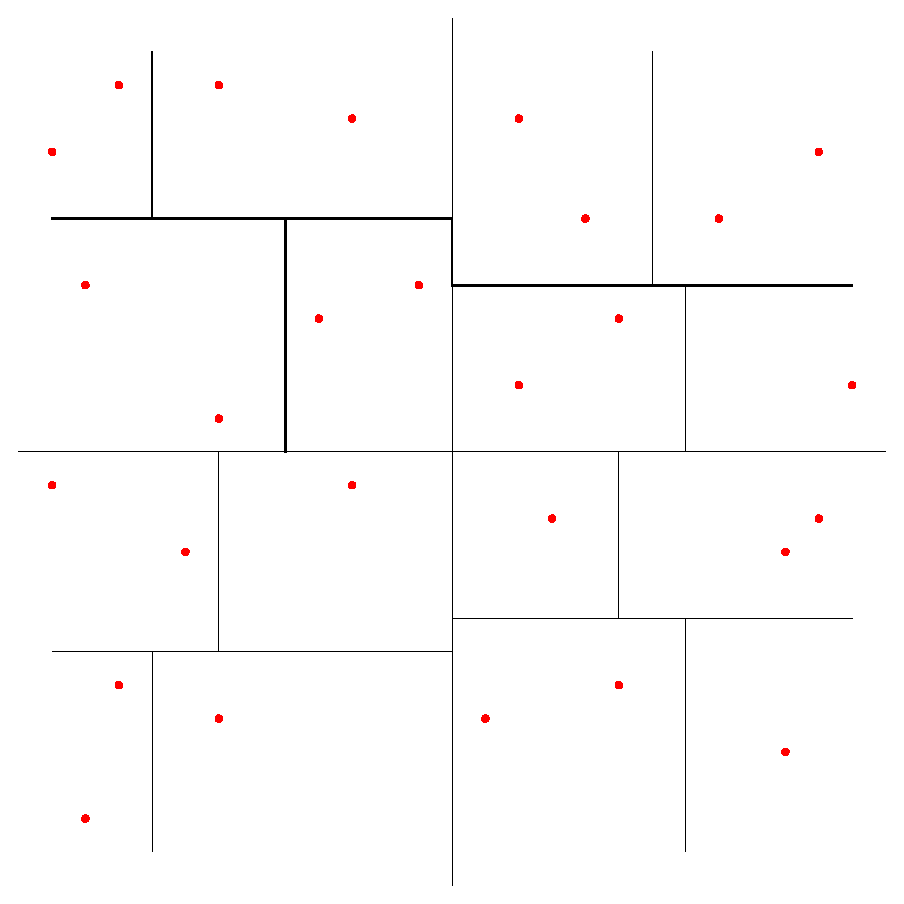
\includegraphics[width=8cm]{Figure1}
      		\caption{Storing whole area covered by nodes}
  				\label{fig:covered}
        \end{subfigure}%
        \qquad\qquad\qquad\qquad
        ~ %add desired spacing between images, e. g. ~, \quad, \qquad etc. 
          %(or a blank line to force the subfigure onto a new line)
        \begin{subfigure}[b]{0.4\textwidth}
                \centering
 				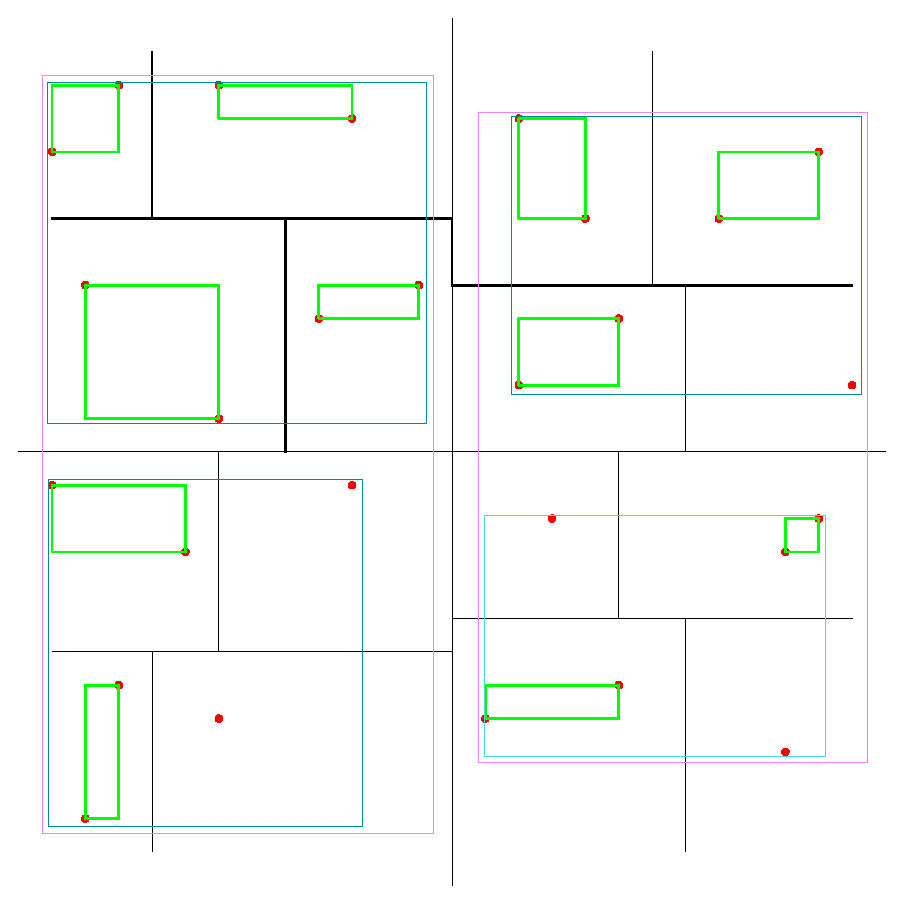
\includegraphics[width=8cm]{Figure2}
 				 \caption{Area covered by points inside nodes}
 				 \label{fig:inside}
        \end{subfigure}
        
\end{figure}

Instead of storing whole area covered by the node (see Figure~\ref{fig:covered}), we could calculate area covered by points inside each node (see Figure~\ref{fig:inside}).

Let us take on example where $k$ points with minimal values of coordinate x are requested. First event contains root of a tree. It is processed. It causes to push two of its sons to the queue. Next, we chose node with smaller minimum value of coordinate x. This event is processed and another two nodes are added. The point with minimal value of coordinate x belongs to exactly one of these nodes and this node is processed. This situation goes on until leaf containing point with a minimum value of coordinate x is processed. At this point we found first point with a minimal value of coordinate x. Then all nodes with lower bound equal to second minimal value of coordinate x are processed. There are again $\Oh(\log n)$ such nodes, all of them are processed and one row is found. The situation goes on until we find $k$ rows.  After finding $k$ points, search process can be stopped and results may be rendered. To sum up, $\Oh(k \log n)$ nodes are added to queue, and $\Oh(k \log n)$ nodes are processed. Finding minimum value of coordinate $x$ of node takes $\Oh(1)$ since we store this information in boundary. Processing one node takes $\Oh(1)$ time. The bootleneck of this solution is priority queue. Priority queue may be implemented as a binary heap. We processed $\Oh(\log n)$ nodes so complexity of this solution is $\Oh(k \log n \log(k \log n))$.

\subsection{Raw pointers instead of shared pointers}

In modern C++ pointers should not be used and shared pointers are recommended instead. The idea behind shared pointer is to automate releasing resources. Basically, shared pointer keeps the counter representing the number of copies of the current pointer. When the shared pointer is created, the counter is incremented. When shared pointer is deleted, the counter is decremented. When the counter is decreased to zero, the resource is released. With such a tool developer is free from most common cause of memory leaks. Unfortunately shared pointers come with time and space overhead. I decided to use raw pointers, which gives better running time. In retrospect, I think it was biggest mistake in the project. The source code became really messy, even small change in legacy code could create bugs.

\subsection{Balancing K-D tree}
K-D tree has similar problem to binary trees. A Binary tree can be unbalanced and so can K-D tree. My idea for balancing K-D tree is very simple. When the number of nodes in one subtree is 2 times larger than the number of nodes in the opposite subtree, I rebuild their parent subtree from scratch.
This is known as partial rebuilding, a simple yet very powerful paradigm often used for making data structures dynamic, for example in weight-balanced trees~\cite{ALPHATREES}. While the worst case complexity of a single operations can be large because of this rebalancing, the amortized complexity is actually rather good. Amortized complexity describes average time required to perform a sequence of related operations. A detailed description with examples of amortized complexity can be found in ~\cite{AMOR}.

\section{Implementation}

\subsection{HTTP Service}

I decided that it would be best if the search engine could work as simple HTTP server. Every query should be send as HTTP GET request. As a base of HTTP server I used \verb|example2| from \verb|boost::asio| documentation \cite{ASIOHTTP}. In Shuffla configuration file user should define the number of available threads. One of the server's starting procedure is to create all these threads. Every HTTP request is assigned to one of these threads by \verb|boost::asio::ip::tcp::acceptor|. There is another thread for periodical functions. Currently it's invoking only saving snapshots. All dependencies of server starting procedure are presented in Figure~\ref{fig:httpservice}.

\begin{figure}[h!]
\centering
  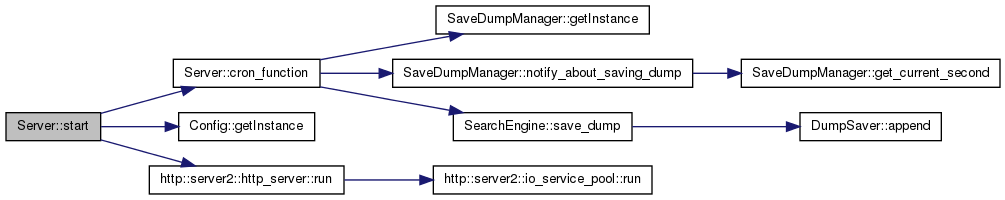
\includegraphics[width=16cm]{start}
  \caption{Processing request begins}
  \label{fig:httpservice}
\end{figure}

\subsection{Validation and passing queries to SearchEngine class}

\verb|http::server2::request_handler::handle_request| passes requesting urls to \verb|QueryDispatcher|. \verb|QueryDispatcher| converts every request to corresponding class by using \verb|QueryCreate|. For instance, the search request is converted to \verb|SearchQuery|, insert is converted to \verb|InsertQuery|, and so on. At this level, syntax validation is performed. In case of an error, HTTP error code 400 is returned and error message is appended to the log file with errors. 

Instances of query classes are sent to \verb|SearchEngine| class. \verb|SearchEngine| class is responsible for:
\begin{enumerate}
\item data validation (types, correspondence to table definition),
\item measuring running time (the engine should report queries being executed for too long),
\item locking tables in case of modifying query,
\item passing valid requests to K-D Trees.
\end{enumerate}

\subsection{Processing insert/delete requests}

Inserting/deleting without tree balancing is pretty straight forward. It is just a simple recursion described in the previous chapter. Balancing is tricky as you may see in dependencies visualisation in Figure~\ref{fig:rebuild}.

\begin{figure}[h!]
\centering
  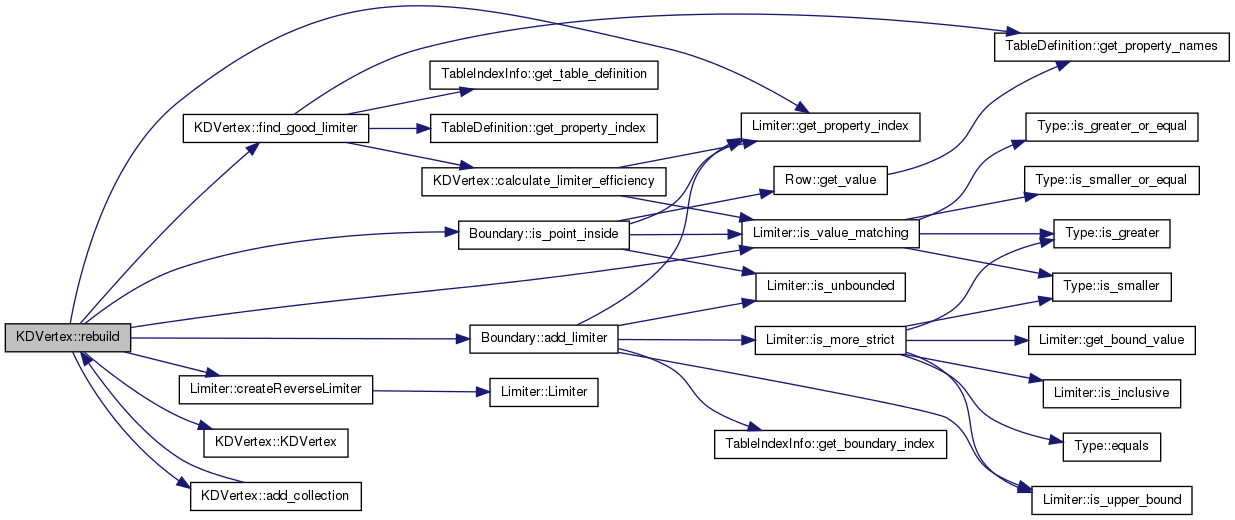
\includegraphics[width=16cm]{rebuild}
  \caption{Rebuilding process}
  \label{fig:rebuild}
\end{figure}

Balancing can be done using any linear algorithm for finding median in the set. I have decided to take a different approach. In \verb|KDVertex::find_good_pivot| I am iterating over all points. Based on coordinate value in currently processed row I create a \verb|Pivot|. \verb|Pivot| is a simple class which takes \verb|Row| and \verb|property_name|. For any \verb|Row|, \verb|pivot| can check if given \verb|Row| satisfy condition defined inside \verb|Pivot|. Algorithm iterates over 20 randomly selected rows in node and in linear time calculates pivot efficiency. If pivot efficiency is good enough (See definition of a well-balanced tree) I stop calculations. If none of these rows create good pivots, I iterate over all rows and check them one by one if they creating good pivot. After selecting pivot I am recursively rebuilding two subtrees. I have decided to use this solution because of space efficiency which is $\Oh(1)$. Space complexity is crucial because if it reaches linear, the rebuilding root may cause memory usage to double. Such a behaviour is very unwelcome in server environment. The implemented solution is $\Oh(n^2)$ but in average case it works well because $\frac{1}{5}$ of rows create good pivots. Therefore, the expected complexity of rebuilding subtree with n nodes is $\Oh(n \log n)$.

\subsection{Processing search requests}

\begin{figure}
\centering
  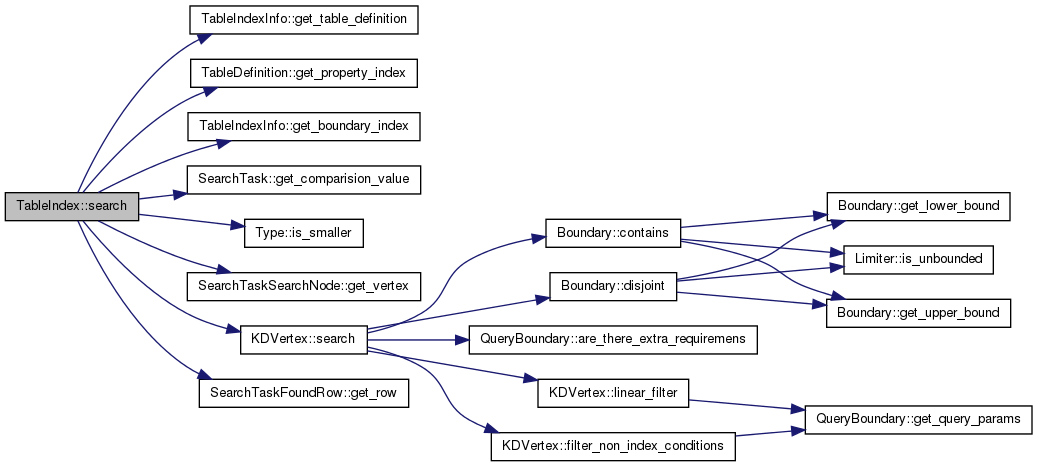
\includegraphics[width=16cm]{search}
  \caption{Processing search request}
  \label{fig:search}
\end{figure}

When request data is validated, control is passed to \verb|TableIndex| class. Actual computations begin here. Let us look at processing search request. Method \verb|TableIndex::search| contains priority queue which processes all search events. There are different objects for different tasks. There is \verb|SearchTaskSearchNode| which contains node to process. There is also \verb|SearchTaskFoundRow| which always contains one row. This row may be inserted to task queue if and only if it satisfies all conditions defined in the search request. Both these classes extend abstract class \verb|SearchTask|. When processing \verb|SearchTaskFoundRow|, algorithm just adds row to the result set. When processing \verb|SearchTaskSearchNode| algorithm passes control to \verb|KDVertex::search|, which returns all events that should be added to the queue. \verb|KDVertex::search| checks if boundary defined by query is disjoint with current node boundary. If it is disjoint, there is nothing more to do. If not, the algorithm simply adds two sons of current node to the queue.

There was an idea to add possibility of multiple index creation. Such index could be created for some subset of the table's properties. Queries with conditions containing only properties from such subset would run much faster. For this feature I introduced two functions \verb|KDVertex:filter_non_index_conditions| \verb|QueryBoundary::are_there_extra_requirements|. Possibility of creating additional indexes is not implemented yet.  

Dependencies of the searching process are visualized in Figure~\ref{fig:search}.

\subsection{Locking tables}

To correct work in multi-threaded environment we must ensure thread safety. It requires from us to eliminate all data races, especially simultaneous writes which can make our data inconsistent. That is why I introduced locking. Basically, by acquiring lock we are restricting access to some part of the code. 

Our goal is to create the following schema: Any number of read-only queries can be run concurrently as long as no write query is being performed at the time. Write queries can be performed if no other query is being performed at the same time. 

The advantage of this locking schema is that it can be implemented using only \verb|mutexes| and \verb|locks| from \verb|boost|. A \verb|mutex| object facilitates protection against data races and allows thread-safe synchronization of data between threads. A thread obtains ownership of a mutex object by calling one of the lock functions and relinquishes ownership by calling the corresponding unlock function. Mutexes may be either recursive or non-recursive and may grant simultaneous ownership to one or many threads. \verb|Boost.Thread| supplies mutexes with exclusive ownership semantics, along with a shared ownership (multiple-reader or single-writer) mutex.
There are three most common kinds of locks. All locks work in a similar fashion. Mutex is passed as a constructor parameter to lock. Ownership of mutex is acquired in a constructor. Ownership of mutex is released when the lock object is destroyed.  

\begin{enumerate}
\item \verb|unique_lock| - When mutex is acquired by \verb|unique_lock|, no one can acquire this lock until unique lock releases ownership of mutex. 
\item \verb|shared_lock| - Multiple shared locks can acquire the same mutex.
\item \verb|upgrade_lock| - Acquires upgradable ownership. Upgradable ownership may be at any time upgraded from shared lock to unique lock and vice versa.
\end{enumerate}

My solution requires every table to have its own mutex. Read-only request uses \verb|shared_lock| and write request uses \verb|unique_lock|. With such solution write queries cannot be executed along with other queries. Using \verb|shared_lock| allows simultaneous execution of other read-only queries. So everything works exactly as it supposed to.

\subsection{How data is stored}

Architecture of data storage in databases is very important. It influences application performance and architecture of all other components. Here are the requirements for data storage: 
\begin{enumerate}
\item all data must be serializable,
\item chosen architecture should force type safety,
\item very good space efficiency,
\item it must be fast!
\end{enumerate}
Values can be strings or numbers, therefore I created 3 classes:
\begin{enumerate}
\item abstract class \verb|Type|,
\item class \verb|TypeString| which extends \verb|Type|,
\item class \verb|TypeNumber| which extends \verb|Type|.
\end{enumerate}

If we take a closer look at specification we may notice that we never change values of existing numbers and strings. Therefore these classes may be immutable. Immutable object is an object whose state cannot be modified after it is created. Immutability trivially guarantees thread-safety and allows for some storage optimization. Let us take a look at \verb|TypeString|. Storing text values in \verb|std::string| would be inefficient because of overhead caused by \verb|std::string| being not immutable. A text is actually stored in \verb|char*|. This array is created in \verb|TypeString| constructor because at this point we know the text length.   

Both \verb|TypeString| and \verb|TypeNumber| implement all supported functions. \verb|TypeNumber| implements equality check, inequalities and strict inequalities. \verb|TypeString| implements equality check, inequalities, strict inequalities, substring and prefix function. Pattern matching is done by function \verb|strstr| from \verb|cstring| \cite{STRSTR}.

Single row stores pointer to the table definition. Apart from that, there is a \verb|std::vector<Type>|, which stores values of all fields.

\subsection{Database persistence}

In case of a crash there must be a way to restore database. In this chapter I will describe how Shuffla preserves data. Guaranteeing persistence of database which holds data in RAM is difficult (as you can see in the example of Redis ~\cite{REDPE}). After every modifying query, engine should not only write such data to disk but ensure that OS will actually write such data to disk. It is a very costly operation which drastically decreases application speed. Instead of such solution, a preferred way is to have “almost durable” system.
Nowadays, there are two most popular ways of having almost durable database in RAM:

\begin{enumerate}
\item AOF - append only file, every modifying query is saved to disk (without forcing OS to actually do it),
\item Snapshotting - in constant time intervals snapshots of database are saved to disk.
\end{enumerate}
I implemented both possibilities. 

\subsection{Presenting results}

Presenting results may sound like a trivial issue. Actually it is not and hardly any libraries would fit for requirements presented below. Modern databases and search engines have to support most popular formats. Nowadays these are JSON, XML and (maybe) YAML. Chosen library should provide the same interface for feeding data to render, without any assumptions of the selected output format. Support for unicode characters is necessary. For some simple queries rendering response could be a bottleneck. That is why I chose \verb|boost::property_tree|. This library does not support unicode by default. It is possible to fix it by following \cite{SOANS} .

\section{Complexities}

Terminology:
\begin{enumerate}
\item $\leftSon(v)$ - left subtree of vertex $v$
\item $\rightSon(v)$ - right subtree of vertex $v$
\end{enumerate}

$n$ stands for the number of points in the tree. Tree $T$ is $\alpha$-balanced if and only if 
$$\displaystyle\mathop{\bigforall}_{v\in T} \quad \frac{1}{\alpha} \leq \frac{|\leftSon(v)|}{|\rightSon(v)|} \leq \alpha$$

The tree is well-balanced if it is 2-balanced and super-balanced if it is  $\frac{3}{2}$-balanced. The height of both well and super balanced trees is $\Oh(\log n)$. Every point belongs to $\Oh(\log n)$ nodes. 

Assumptions:
\begin{enumerate}
\item all values of all columns are unique
\item rebuilding the subtree with root $\theta$ causes the subtree to be super-balanced.
\end{enumerate}

\subsection{Inserting/deleting point $X$}

\begin{lemma}\label{lem:1}
Rebuilding tree of size $n$ takes $\Oh(n \log n)$.
\end{lemma}

\begin{proof}
We can find the median in linear time~\cite{FIVE}. Hence, in order to rebuild a tree, we first find the median and then, recursively, rebuild two subtrees. Complexity of such procedure can be described by $T(n)=\Oh(n)+T(\alpha n)+T((1-\alpha)n)$, where $\frac{2}{5}\leq \alpha \leq \frac{3}{5}$. The recurrence solves to $T(n)=\Theta(n\log n)$. This can be proved by drawing recurrence call tree. At each level the work done sums to $\Oh(n)$. There are $\Oh(\log n)$ levels, therefore the complexity is $\Oh(n \log n)$.
\end{proof}

\begin{lemma}\label{lem:2}
Amortized time of insert/delete is $\Oh(\log^2 n)$.
\end{lemma}

\begin{proof}

We will give $6\log n$ credits to each node visited during insert/delete. As the depth of the whole tree is $\Oh(\log n)$, the total number of credits allocated during a single insert/delete operation is just $\Oh(\log^{2}n)$. The goal is to make sure that the following invariant holds: a node such that the left subtree is of size $n_{l}$ and the right subtree is of size $n_{r}$ has at least $6|n_{l}-n_{r}|\log n$ credits available (observe that because the tree is well-balanced this is at most $n\log n$). We must prove that the invariant still holds after each insert/delete and that we always have enough credits to amortize the rebuilding. I will consider those two parts separately.

\begin{enumerate}

\item Each node visited during an insert/delete operation gets $6\log n$ credits. Notice that after the visit we either increase or decrease $n_{l}$ or $n_{r}$. Hence, we increase $6|n_{l}-n_{r}|\log n$ by at most $6\log n$ and so we can afford to pay for this increase using the new credits allocated to the node (it can also happen that we decrease $|n_{l}-n_{r}|\log n$, which is even better).

\item We rebuild a node as soon as one subtree is two times larger than the other, say $n_{l} = 2n_{r}$. Then the number of credits accumulated at the node is at least 6($2n_{r}-\frac{3}{2}n_{r}
)\log n = 6\frac{1}{2}n_{r}\log n = n\log n$, where $n=n_{l}+n_{r}$. After we reconstruct the tree, the required number of credits will be at most $\log n$. Hence, we can use $(n-1)\log n$ credits to pay for the reconstruction and by Lemma~\ref{lem:1} this is enough.

\end{enumerate}

There is one additional detail. The value of $\log n$ can (and will) actually change during the execution of the algorithm. Its integer part is actually important. In order for it to increase, we need to perform $n$ insert/delete operations. Hence, if we charge each such operation with additional $c\log^{2} n$ credits, whenever the integer part of $\log n$ increases, we will have $cn\log^{2} n$ credits available. 

Now, for each node of the tree we need to add $n\log n$ credits, hence the total required number of credits is described by the recurrence $T(n)=n\log n+T(\alpha n)+T((1-\alpha)n)$, where $\frac{1}{3}\leq \alpha \leq \frac{2}{3}$. The recurrence solves to $T(n)=\Theta(n\log^{2}n)$. This can be proved by drawing recurrence call tree. At each level the work done sums to $\Oh(n \log n)$. There are $\Oh(\log n)$ levels, therefore the complexity is $\Oh(n \log^2 n)$.

We have enough credits to pay for the increase.
\end{proof}

\subsection{Search}

Recall that the complexity of searching in a static K-D tree is $\Oh(n^{1-1/d} + k)$. Unfortunately, such worst case bound seems difficult to achieve in our dynamic settings, where the tree is just well-balanced. Nevertheless, a slightly weaker bound holds under the assumption that a child of a node corresponding to $n$ points corresponds to at most $\frac{2}{3}n$ points itself.

\begin{lemma}\label{lem:3}
Upper bound for number of processed nodes on level $d$ is $2^{d-1}$.
\end{lemma}

\begin{proof}

K-d tree is a binary tree. Root has height 0, its children have height 1, and so on. Let me count maximal possible number of visited nodes on level $d$ by a recursive search algorithm where region is defined by $X_e$ $\geq$ $C$. A node will be recursively processed iff it intersects search region but is not fully contained in it. At one of these levels there will be a pivot on dimension $e$. Such line intersects either the region represented by left son or right son, not both. Therefore, only one of its sons will be recursively called. Then the upper bound for processed nodes is $2^{d-1}$. It can be easily generalized to every region. Adding another condition may only reduce the number of processed nodes. Hence, the upper bound for number of processed nodes on level $d$ is $2^{d-1}$. 
\end{proof}


\begin{lemma}\label{lem:4}
Upper bound for average number of points inside a processed node on level $d$ is $\frac{\frac{2}{3}n}{2^{d-1}}$.
\end{lemma}

\begin{proof}

The total number of points on all nodes on level $d$ is $n$. The total number of points in processed nodes on level $d$ is at most $\frac{2}{3}n$. Worst case scenario occurs when the number of processed nodes is maximal. From proof of lemma ~\ref{lem:3} we know that it is the scenario with search region defined as $X_e$ $\geq$ $C$. For all nodes with pivots on dimension $e$ it is true that nodes from one son will be processed and nodes from the other son will not be processed. Tree is well-balanced so ratio between processed points and not precessed points is not greater than 2:1. Hence, the upper bound for average number of points inside a processed node on level $d$ is $\frac{\frac{2}{3}n}{2^{d-1}}$.
\end{proof}

I will prove that the worst case scenario occurs when all subproblems are the same size. Then the complexity will be $T(n)=2^{d-1}T(\frac{\frac{2}{3}n}{2^{d-1}})$.

\begin{lemma}\label{lem:5}
The recurrence describing the worst-case scenario is $T(n)=1+2^{d-1}T(\frac{\frac{2}{3}n}{2^{d-1}})$ which solves to $\Oh(n^{1 - \log_{3*2^{d-2}}{\frac{3}{2}}})$.
\end{lemma}

\begin{proof}

My goal is to prove that $T(n) \leq c n^a$ for some constant $a < 1$ using induction on $n$. For small values of $n$ it is true because we can choose constant $c$. Now let me prove that $T(n) \leq c n^a$ assuming that $T(n') \leq c n'^a$ for all $n'<n$. We have:

$$T(n) = \displaystyle\sum\limits_{i=1}^{2^{d-1}} T(x_i)\leq\displaystyle\sum\limits_{i=1}^{2^{d-1}} c(x_i)^{a}  \quad\text{where}\quad  \displaystyle\sum\limits_{i=1}^{2^{d-1}} x_i = \frac{2}{3}n$$ 

As we are interested in upperbounding $T(n)$, we are interested in the maximum possible value of the sum of all $(x_i)^{a}$ under the condition that all $x_{i}$ sum up to $\frac{2}{3}n$. Because the function $f(x)=x^{a}$ is convex for $a<1$, from Jensen's inequality we get that the sum is maximized when all $x_{i}$ are equal. Hence:

\begin{eqnarray*}
T(n) &=& \displaystyle\sum\limits_{i=1}^{2^{d-1}} T(x_i) = 2^{d-1} T\left(\frac{\frac{2}{3}n}{2^{d-1}}\right) \leq 2^{d-1} c \left(\frac{\frac{2}{3}n}{2^{d-1}}\right) ^ a  \\
& = & c 2^{d-1} \left(\frac{2}{3}\right)^a 2^{-a(d-1)} n^a = 2^{(1-a)(d-1)} \left(\frac{2}{3}\right)^a c n^a
\end{eqnarray*}

Hence $T(n)\leq c n^{a}$ as long as $2^{(1-a)(d-1)} (\frac{2}{3})^a \leq 1$.
\bigskip


Simple transformations of $2^{(1-a)(d-1)} (\frac{2}{3})^a \leq 1$ gives $\frac{d-1}{\log_2{3} + d - 2} < 1$ so for all d exists a < 1.

\end{proof}

$T(n)=1+2^{d-1}T(\frac{\frac{2}{3}n}{2^{d-1}})$ solves to (by the master theorem) $T(n)=\Oh(n^{\frac{\log 2^{d-1}}{\log 3*2^{d-2}}})$.

\begin{eqnarray*}
\frac{\log 2^{d-1}}{\log 3*2^{d-2}} = \log_{3*2^{d-2}}{2^{d-1}} = \log_{3*2^{d-2}}{2^{d-1}} + \log_{3*2^{d-2}}{\frac{3}{2}} - \log_{3*2^{d-2}}{\frac{3}{2}} = \\ \log_{3*2^{d-2}}{3*2^{d-2}} - \log_{3*2^{d-2}}{\frac{3}{2}} = 1 - \log_{3*2^{d-2}}{\frac{3}{2}}
\end{eqnarray*}

Therefore $T(n) = \Oh(n^{1 - \log_{3*2^{d-2}}{\frac{3}{2}}})$.
Here is table with a few values of d and complexity associated with this d.
\bigskip

\noindent\makebox[\textwidth]{%
\bigskip
\begin{tabular}{|l|c|}
\hline d & Complexity \\
\hline 2 & $\Oh(n^{0.631})$ \\
\hline 3 & $\Oh(n^{0.774})$  \\
\hline 4 & $\Oh(n^{0.837})$ \\
\hline 6 & $\Oh(n^{0.896})$ \\
\hline 10 & $\Oh(n^{0.939})$ \\
\hline 
\end{tabular}
}

\bigskip
While the worst case bound might seem somehow disappointing when $d$ is large, one should remember that in practice we will observe a much better performance. For average queries without substring conditions algorithm behaves like $\Oh(S \log n)$ where S = offset + limit.

Let me explain that by taking data with random distribution. When algorithm recursively enters node of K-D tree, with some probability there are some rows fitting query. Algorithm will find some results if there is a point on intersection of search region and region representing the node. Probability of such event for search region $S$ and region $R$ representing node can be defined as $P(S, R) = 1 - (\frac{|S \cap R|}{|R|})^p$ where $p$ is the number of points inside $R$. This number may be small only if $|S \cap R|$ is very small compared to $|R|$. If we bound this probability by a constant, finding single row takes $\Oh(\log n)$.

\section{Tested engines}

All engines must be tested on the same schema and by the same queries. Yet presented engines have different syntax. In chapters below I will describe table configurations and how queries were translated during their testing.
\subsection{Solr}

During tests I was using Solr 3.6.1. Tables in Solr are defined via xml file called schema.xml. Part of this file responsible for creating table is listed below.

\begin{verbatim}
<fields>
  <field name="id" type="uuid" indexed="true" stored="true" default="NEW"/>
   <field name="first_name" type="text_general" indexed="true"
             stored="true" required="true" /> 
   <field name="last_name" type="text_general" indexed="true" 
             stored="true" required="true"/>
   <field name="age" type="int" indexed="true" stored="true" /> 
   <field name="city" type="text_general" indexed="true" stored="true"/>
</fields>

<uniqueKey>id</uniqueKey> 
\end{verbatim}

Solr requires a unique key. Combining all properties is not enough. For example there are lots of men named Jan Kowalski in Warsaw. Therefore, I created another property named id.

\bigskip
Here is the syntax for all types of queries:
\begin{enumerate}
\item Equality check: \verb|property:value|
\item Inequalities are realized by range queries: \verb|property:[from TO to]|. \verb|From| and \verb|to| can be replaced by \verb|*|. For example searching number greater then or equal to 2 is performed by \verb|property:[2 TO *]|. \verb|property:[* TO *]| matches everything.
\item Strict inequalities are realized by excluding some range \verb|-property:[from TO to]|. For example searching numbers smaller than 2 is performed by excluding range [2,$\infty$]: \verb|-property:[2 TO *]|.
\item Prefix queries: \verb|property:value*|.
\item Substring queries: \verb|property:*value*|.
 
\end{enumerate}

\subsection{PostgreSQL}

I am using PostgreSQL 9.1. Schema used in testing is:

\begin{verbatim}
CREATE TABLE users (
  first_name TEXT not null,
  last_name TEXT not null,
  age INT not null,
  city TEXT not null
);

CREATE INDEX index1 ON users (first_name, last_name, age, city);
CREATE INDEX index2 ON users (last_name, age, city);
CREATE INDEX index3 ON users (city, age, first_name);
CREATE INDEX index4 ON users (age, first_name, last_name);
\end{verbatim}

Syntax:
\begin{enumerate}
\item Equality check, inequalities and strict inequalities are realized by \verb|=|, \verb|>=|, \verb|<=|, \verb|>|, \verb|<|
\item Prefix queries are handled by \verb|property LIKE "text%"|
\item Substring queries are handled by \verb|property LIKE "%text%"|
\end{enumerate}

For text-search PostgreSQL implemented special type of indexes: GIN \cite{PSQLGIN} and GIST \cite{PSQLGIST}. Unfortunately I was unsuccessful in making them work with Polish words. Therefore I tested PostgreSQL with default indexes.

\subsection{Shuffla}

Table is created by sending HTTP request:
\begin{verbatim}
/create_table/test_table/?first_name=string&last_name=string&age=int&city=string
\end{verbatim}
Shuffla's query format is:

\begin{verbatim}
/search/<table name>/?subquery(&subquery)*
\end{verbatim}
Where subquery can be:
\begin{enumerate}
\item \verb|field|=\verb|value| for equality check
\item \verb|GREATER_THAN|(\verb|field|)=\verb|value| means that given value must be greater than value of \verb|field| 
\item \verb|SMALLER_THAN|, \verb|SMALLER_OR_EQUAL|, \verb|GREATER_OR_EQUAL| work in similar fashion to \verb|GREATER_THAN|
\item \verb|PREFIX|(\verb|field|)=\verb|value| requires \verb|field| to have prefix \verb|value|
\item \verb|CONTAINS|(\verb|field|)=\verb|value| requires \verb|field| to contain \verb|value| as a substring
\end{enumerate}

\section{Tested results}

\subsection{How results are tested}

Testing environment is a machine with Intel i5-2500 processor (4 cores, 3.5GHz), 8GB RAM and SSD drive. Comparing engines with default settings is pointless. I have tried to configure them all to production use. The most important change is increased memory limit for Solr and PostgreSQL to 1GB.

In nk we have got several millions of registered users. This number does not grow in spectacular fashion. I want to simulate engines behaviour in similar conditions. 

At the beginning I inserting $8 * 10^6$ randomly generated users. Then I will run a script which creates random insert/search queries. It sends created queries for few hours and calculates statistics.

Inserted data is generated in a very simple way. I have gathered lists of most popular first and last names in Poland (with counts). The probability of selecting a name is proportional to its count. The age is selected with linear distribution from set $[5, 100]$. 

Search queries are generated by following procedure:
\begin{enumerate}
\item Pick N - number of expressions in search query
\item The column in expression is selected from a set [first name, last name, age, city]. Each of them has 25 percent chance to be chosen.
\item If selected column has int type (only age is an integer), the possible queries are equality check, inequalities and strict inequalities. Each of them has 20 percent chance to be chosen.
\item If selected column has string type, the possible queries are comparison, inequalities, prefix queries and substring queries. Prefix and substring queries have 25 percent chance to be chosen. Each of the remaining conditions has 10 percent chance to be chosen. The selected column is always compared to another string. This string is selected by selecting a random word with 1 to 5 characters.
\end{enumerate}

Then I will select random column and I will set it as order by column. Then I will choose offset and limit from range $[0, 50]$.

\subsection{Inserting 8 million rows}

The average length of combined \verb|first_name|, \verb|last_name|, \verb|city| fields contains 21 characters. It means that the size of inserted data is about 250 MB. There is always some overhead of keeping data in data structures. It causes shuffla to use 6 GB RAM.

Inserting 8 million rows is not the most important part of testing. It is performed before production deployment and I will do this part only once. I am happy as long as indexing time does not last longer than a few hours. 

Shuffla handles insert requests with speed of hunderds requests per second. Using single inserts with other engines is not so efficient. All considered engines are able to read csv file and import data from such file. For them it is the only way to import data within few hours.

\subsection{Statistics}

For the purpose of testing in true multi-threaded environment I used tsung. Tsung is a distributed load testing tool written in erlang. It is protocol-independent and can be used to stress HTTP, WebDAV, SOAP, PostgreSQL, MySQL, LDAP, and Jabber/XMPP servers. 

I have used 4 core processor for testing so I decided to test all engines using 4 threads. Each thread sends 10.000 randomly created queries. 

Solr and PostgreSQL use less than 1 GB of RAM. It is possible because both these engines keep data on a hard drive. Shuffla stores everything in RAM and consumes 6GB of RAM. 

\begin{figure}[h!]
\centering
  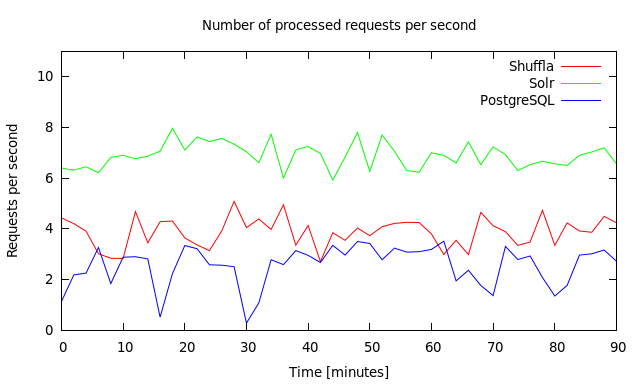
\includegraphics[width=12cm]{request_count_tn}
  \label{fig:request_count_tn}
\end{figure}

\noindent\makebox[\textwidth]{%
\begin{tabular}{|l|c|c|c|c|}
\hline Engine & Req / sec & Memory consumption \\
\hline Solr & 6.89 & 1GB \\
\hline Shuffla & 3.86 & 6GB  \\
\hline PostgreSQL & 2.55 & 1GB \\
\hline 
\end{tabular}
}

\bigskip

Solr is superior over Shuffla in every way. Solr is faster. It uses less memory. It is more configurable, we could for example increase Solr memory limit. Solr is just better option, especially for large social website purposes. 

\section{Few words about Solr in nk}

\subsection{Search architecture in nk}

\begin{figure}
\centering
  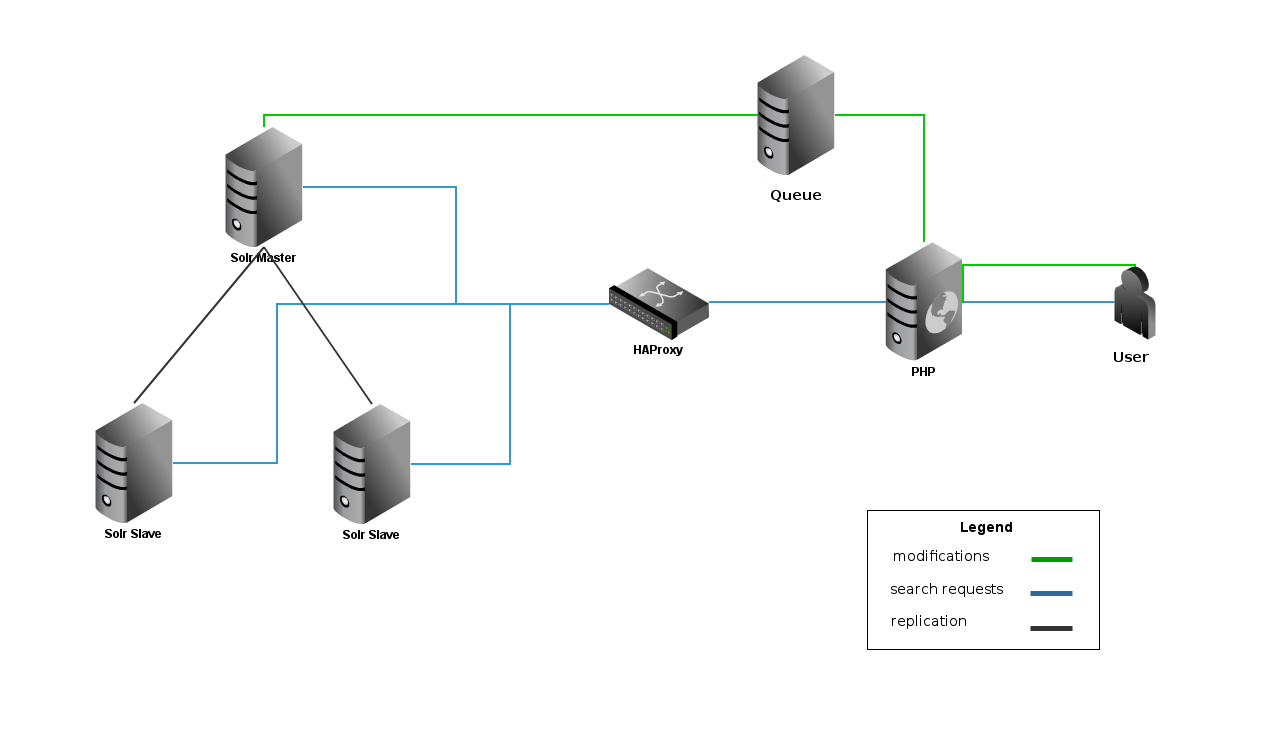
\includegraphics[width=12cm]{architektura_wyszukiwania}
  \caption{Architecture of searching}
  \label{fig:architektura_wyszukiwania}
\end{figure}

In nk we have 3 servers with Solr. There is master-slave replication between them. One server is a master, another two others are slaves. Only master processes modifying queries. When user does anything related to searching, PHP code handles it.

When some action requires modifying data in Solr, PHP code creates task for it. This task is inserted into a queue. There is a background job which processes all tasks from queue one by one. We need queue to avoid unexpected spikes. For example, the uncaught spammer attack may cause 1000 modifying requests per second \footnote{Actually this is highly unlikely, nk crashes spammers activity extremely well}. If this happens, master could easily crash or at least experience some kind of slowness due to a big load. We want to avoid such situations. 

In case of search request we need to distribute requests between servers. For this purpose the search requests go through HAProxy \cite{HAPROXY}. This load balancer is distributes requests between our 3 servers.

\subsection{Statistics from master server}

\begin{figure}
        \centering
        \begin{subfigure}[b]{0.45\textwidth}
                \centering
                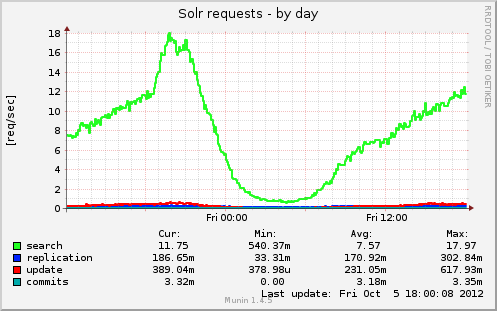
\includegraphics[width=\textwidth]{solr_users_reqs-day}
                \label{fig:solr_users_reqs-day}
        \end{subfigure}%
        ~ %add desired spacing between images, e. g. ~, \quad, \qquad etc. 
          %(or a blank line to force the subfigure onto a new line)
        \begin{subfigure}[b]{0.45\textwidth}
                \centering
                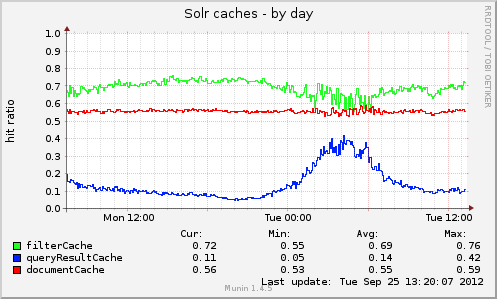
\includegraphics[width=\textwidth]{solr_users_cache-day}
                \label{fig:solr_users_cache-day}
        \end{subfigure}
        
        \label{fig:animals}
        
        \centering
        \begin{subfigure}[b]{0.45\textwidth}
                \centering
                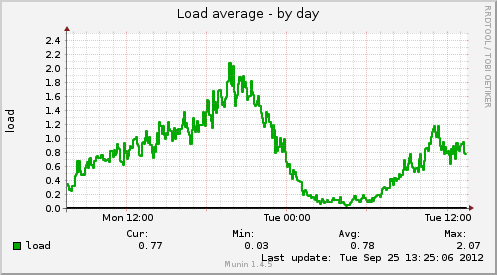
\includegraphics[width=\textwidth]{load-day}
                \label{fig:load-day}
        \end{subfigure}%
        ~ %add desired spacing between images, e. g. ~, \quad, \qquad etc. 
          %(or a blank line to force the subfigure onto a new line)
        \begin{subfigure}[b]{0.45\textwidth}
                \centering
                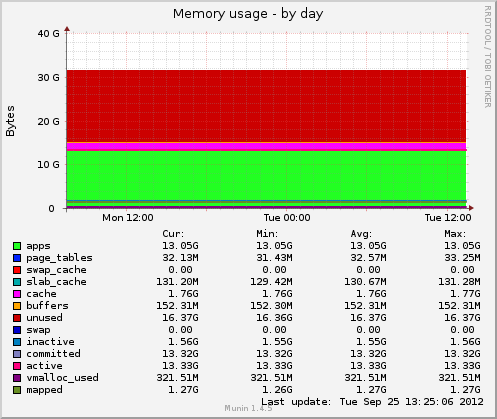
\includegraphics[width=\textwidth]{memory-day}
                \label{fig:memory-day}
        \end{subfigure}
        
        \label{fig:animals}
        
        \centering
        \begin{subfigure}[b]{0.45\textwidth}
                \centering
                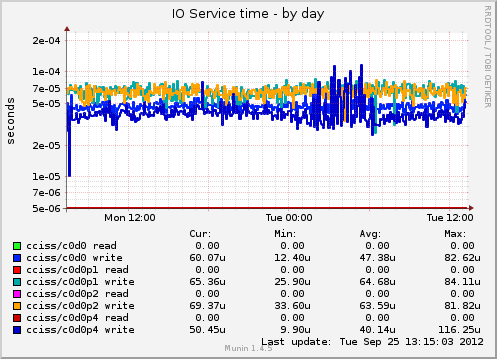
\includegraphics[width=\textwidth]{iostat_ios-day}
                \label{fig:iostat_ios-day}
        \end{subfigure}%
        ~ %add desired spacing between images, e. g. ~, \quad, \qquad etc. 
          %(or a blank line to force the subfigure onto a new line)
        \begin{subfigure}[b]{0.45\textwidth}
                \centering
                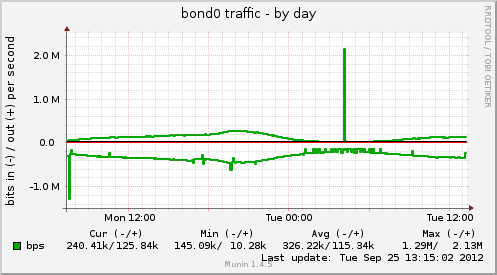
\includegraphics[width=\textwidth]{if_bond0-day}
                \label{fig:if_bond0-day}
        \end{subfigure}
        
        \label{fig:animals}
        
        \centering
        \begin{subfigure}[b]{0.45\textwidth}
                \centering
                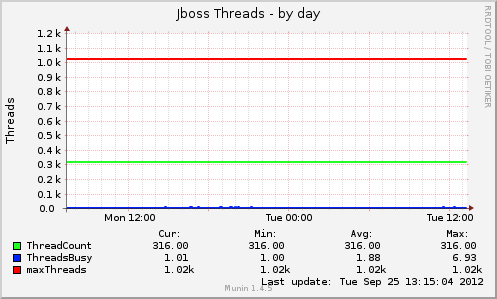
\includegraphics[width=\textwidth]{jboss_threads-day}
                \label{fig:jboss_threads-day}
        \end{subfigure}%
        ~ %add desired spacing between images, e. g. ~, \quad, \qquad etc. 
          %(or a blank line to force the subfigure onto a new line)
        \begin{subfigure}[b]{0.45\textwidth}
                \centering
                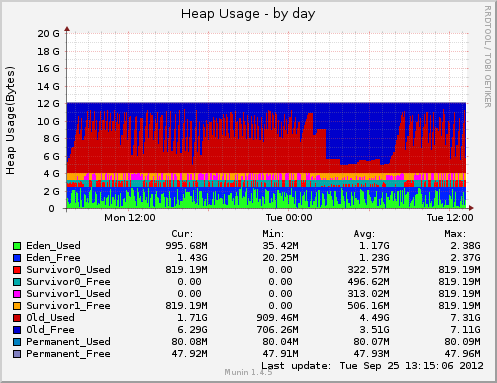
\includegraphics[width=\textwidth]{jstat__heap-day}
                \label{fig:jstat__heap-day}
        \end{subfigure}
        
        \label{fig:animals}
\end{figure}

\subsubsection*{Number of requests, load - by day} 
At night Solr does not do much. The load grows as the day progresses. At the peek (about 8 PM) our master server handles 18 search requests per second. the number of other requests like updates/replication/commit is negligible. One might not forget that we have three Solr servers on production and this chart is only from one of them. A load is a measure of the amount of computational work that a computer system performs. \jarek{Zdanie z wiki} Load $X$ means that we need at least $\lceil X \rceil$ CPUs to run all processes without any of them waiting for a turn. 

\subsubsection*{Memory, heap usage}
At nk we use half of available memory because the other half is reserved for unexpected events, for example, a crash of one server. It may require increasing memory limits on two other machines. Java on our production environment is executed with \verb|-Xms24G -Xmx24G|, which means that memory used by heap plus memory used by stack cannot exceed 24GB. You may find our heap usage very strange. Most of heap memory is used by caches. We commit changes every 15 minutes, which causes all caches to be flushed. For another 15 minutes cache is filling (by processing search queries) and then flushed again.

\subsubsection*{Disk usage and network traffic statistics}
IO Service shows average values of how much time a disk works during a second. It shows very small values. On production all Solr data is kept on ramdisks. It is not zero because of the work done by operating system. Solr network traffic is not huge, it rarely reaches 1 megabit. In the evening, we reach a peek with more than a 100 simultaneous connections from PHP servers to Solr.


\subsubsection*{JBoss threads}
Solr must be executed by some application container. For this purpose we chose JBoss. Thread pool contains more than 300 threads. Usually only small amount of this number is used.

\subsubsection*{Cache usage}
Solr has advanced cache system. Usually about 70 percent of requests are rendered based on values from cache.  At night there is a small number of requests and Solr is unable to get passed warming stage before next commit.  Hit ratio is slightly smaller, about 60 percent at night.

\section{Summary}

After this discussion it might seem that Shuffla is useless. I have to disagree. Shuffla fits great for smaller projects like searching through internet forum or a blog. Both Solr and PostgreSQL require quite difficult installation and configuration. Installation of shuffla takes 2 minutes, creating table takes 10 seconds and searching is very easy. In short/simple projects having possibility of integrating search engine in less than 5 minutes is more than welcome.

%%%%%%%%%%%%%%%%%%%%%%%%%%%%%%%%%%%%%%%%%%%%%%%%%%

\bibliographystyle{abbrv}
\bibliography{biblio}

\end{document}

%%%%%%%%%%%%%%%%%%%%%%%%%%%%%%%%%%%%%%%%%%%%%%%%%%